\documentclass[12pt,a4paper]{article}
\usepackage[utf8x]{inputenc}
\usepackage{ucs}
\usepackage[spanish]{babel}
\usepackage{amsmath}
\usepackage{amsfonts}
\usepackage{amssymb}
\usepackage{makeidx}
\usepackage{graphicx}
\usepackage{lmodern}
\usepackage{kpfonts}
\usepackage{fourier}
\usepackage[left=2cm,right=2cm,top=2cm,bottom=2cm]{geometry}
\author{Grupo }
\begin{document}
\begin{center}
\section*{UNIVERSIDAD DE GUAYAQUIL}
\section*{FACULTAD DE CIENCIAS MATEMÁTICAS Y FÍSICA}
\section*{CARRERA DE INGENIERÍA DE SOFTWARE}

\includegraphics[scale=0.3]{UGlogo.png}  
\section*{INTEGRANTES}
\subsubsection*{DOMINGUEZ KEVIN\\SOTOMAYOR KEVIN\\QUISNANCELA OSCAR}
\section*{PARELELO}
\subsubsection*{SOF-S-MA-3-2}
\section*{DOCENTE\\ING. MIGUEL BOTTO TOBAR}
\end{center}
\newpage
\section*{Análisis - Aplicación de Norma ISO 9001}
\section{Programa: Software de aplicación web para la gestión de proyectos de acabados de Obras 
en Gypsum para la Empresa ADT} 
\paragraph*{La aplicación web para la gestión de proyectos de acabados de Obras en Gypsum para la Empresa ADT consiste en registrar datos para el manejo de información por parte del personal administrativo y el supervisor de obras a través de la aplicación web para tomar decisiones sobre la administración en la construcción de estructuras en Gypsum.}
\paragraph{El sistema colabora con el diseño y desarrollo de la programación de una página web que facilita el desempeño de las labores de cotización de la empresa ADT que se dedica al acabado residencial con Gypsum. Las labores de investigación van a ir desde el levantamiento de información en el sitio, recolección de datos, mediante las técnicas adecuadas de entrevista y cuestionarios, para poder establecer la solución más óptima a los problemas que se presentan.}
\section{Referencia normativa}
\paragraph{Esta documentación para su análisis es tomada de una tesis de la universidad de Guayaquil – facultad de Ingeniería Industrial – Carrera Sistemas de Información, octubre del 2019}
\section{Términos y definiciones}
\paragraph{La aplicación web utiliza el termino como un producto de servicio privado solamente para el uso de la empresa y clientes de la misma.}
\section{Sistema de gestión de calidad}
\paragraph{Acerca de la documentación, el software se encuentra debidamente documentado con el fin de mejorar la eficacia continua de la aplicación, con respecto a los requisitos generales hubo entrevistas continuas con el cliente para tomar nota de los requisitos que el aplicativo debía tener como las operaciones que debe realizar el sistema.}
\section{ Responsabilidad de la dirección}
\paragraph{La alta dirección debe proporcionar evidencia de su compromiso con el desarrollo e implementación del sistema de gestión de la calidad, así como con la mejora continua de su eficacia, satisfaciendo las necesidades del cliente para la empresa, llevando a cabo las revisiones en el funcionamiento y disponibilidad de recursos.}
\newpage
\section{Gestión de los recursos}
\paragraph{En el software la gestión, seguimiento y realización de cotizaciones de proyectos de acabados de obras para la empresa ADT. Para la implementación de esta aplicación web, se ha tomado en cuenta el área de administración y proformas de cotizaciones manuales el cual ha contribuido como herramienta de valiosa ayuda para la empresa en general y sus clientes.
Los componentes tecnológicos más idóneos para el diseño del sistema se escogen de acuerdo a diversos factores como precio, utilidad y diseño. A continuación, se detallan los diferentes recursos lógicos y físicos que se necesitaron para el desarrollo de la aplicación:}
\subsubsection{SOFTWARE }
\paragraph{Página web ayuda a gestionar a través de internet, esto conlleva a que se requiera menos recursos de programación, además de ofrecer la ventaja de funcionar en cualquier dispositivo conectado a la web, otra de las alternativas es que no necesito de espacio físico en el disco duro de la máquina que ocupa. Utilizamos PHP que es un lenguaje de código abierto y que es actualizable en HTML, al ser de código abierto implica en que está disponible para todos los clientes de forma gratuita, con un fácil nivel de aprendizaje para su uso, utiliza muchas técnicas de programación orientada a objetos. Framework CSS Bootstrap, conjuntos de herramientas y métodos que ayudan a mejorar la experiencia de desarrollo con CSS, que aportará de gran manera en el diseño de la página web. Con las herramientas de scripts y hojas de estilo sirvieron de apoyo en la aplicación en forma de clases al código HTML. Para el desarrollo del proyecto utilizamos el motor de base de datos MySQL, lenguaje de programación PHP en la versión 7.0, un Hosting con Apache y como IDE NetBeans 8.2.}
\subsubsection{HARDWARE}
\paragraph{Los componentes físicos que se necesitan para el desarrollo de la aplicación según las características técnicas fueron: }
\begin{itemize}

\item Un computador para el diseño con Windows 10.
\item Sistema Operativo de 64 bits.
\item Procesador Intel. 
\item Memoria RAM de 8 GB.
\item Disco Duro de 1TB. 

\end{itemize}

\section{REALIZACIÓN DEL PRODUCTO }
\subsubsection{}
\paragraph{Planificación del producto; el tiempo determinado para la realización del producto fue de aproximadamente 4 meses, que empiezo desde el mes de mayo hasta septiembre del 2019.}
\newpage
\subsubsection{}
\paragraph{Procesos relacionados con el cliente; se procedió a entrevistas directas con el cliente cada semana para recopilar información acerca de lo que debe realizar el sistema y en el levantamiento de información mediante la técnica de observación y entrevistas sobre las empresas dedicadas al acabado de construcciones se constata que un 60 no utilizan recurso tecnológico para administrar el desarrollo de los proyectos asignados, el otro 40 restante, lo hace mediante herramientas informáticas como los procesadores de textos y hojas de cálculo, empleando para ello las características más básicas de cada una de estas herramientas}
\subsubsection{}
\paragraph{Procesos relacionados con el producto; el desarrollo del aplicativo web para la gestión de proyectos de acabados de obras en Gypsum permite tanto al personal administrativo y al supervisor de obras de los contratistas, manejar las mejores técnicas de administración y en conjunto con el control en los procesos de construcción de los proyectos residenciales otorgando calidad, eficiencia, y seguridad en cada uno de los trabajos realizados.}
\section{DISEÑO Y DESARROLLO }
\paragraph{Se procede a diseñar un árbol con sus respectivas funciones tomando en cuenta la problemática en la está la empresa, todo esto a partir de la información tomada de la empresa ADT.}

\begin{figure}[hbtp]
\caption{}
\centering
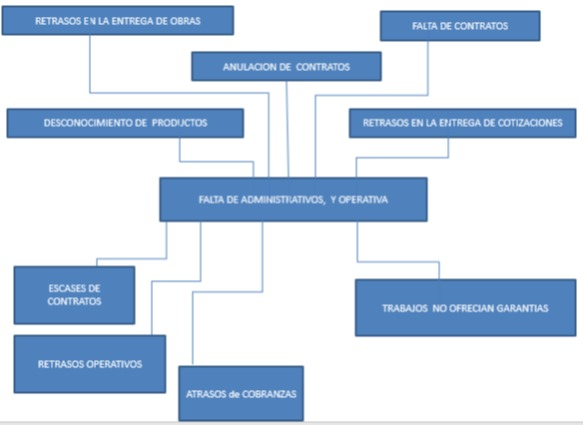
\includegraphics[scale=0.3]{Primera.jpeg}
\end{figure}


\paragraph{
El desarrollo está basado a una programacion orientada a objetos, ya que se requiere tener un control estricto de todo el proyecto a realizar. Trabaja mediante fases, cada fase debe ser presentada claramente, seguida de secuencias, apoyándose en el soporte UML.
Para el desarrollo se implementó el método ICONIX que es una metodología pesada-ligera de Desarrollo del Software que se halla a medio camino entre RUP (Rational Unified Process) y XP (eXtreme Programming), es una metodología simplificada en comparación a otras más tradicionales, la cual unifica un conjunto de métodos de orientación a objetos con el objetivo de tener un control estricto sobre todo el ciclo de vida del producto a realizar, cuenta con una secuencia de pasos que se deben seguir y determina claramente las actividades a desarrollar en cada etapa del ciclo de vida del proyecto que la utilice.}
\newpage

\begin{itemize}
\item Análisis de requisitos: modelo de dominio, prototipos rápidos y modelos de caso de uso. 
\item Análisis y diseño preliminar: descripción de casos de uso y diagrama de robustez. 
\item Diseño: diagrama de secuencia y completar el modelo estático. 
\item Implementar: utilizar un diagrama de componentes, escribir/generar código y realización de pruebas. 
\end{itemize}

\paragraph{El desarrollo del código se implementó en la plataforma Java Enterprise Edition, traducida como Java de Edición Empresarial, para poder realizar y desarrollar programas bajo la plataforma Java, aquí se desarrollan diferentes interfaces de programación de aplicaciones de desarrollo de este lenguaje, y otros servicios de tecnología web, se utilizó el motor de base de datos MySQ, lenguaje de programación PHP en la versión 7.0 y un Hosting con Apache y como IDE NetBeans 8.2}

\section*{LEVANTAMIENTO DE REQUERIMIENTOS}
\begin{figure}[hbtp]
\caption{}
\centering
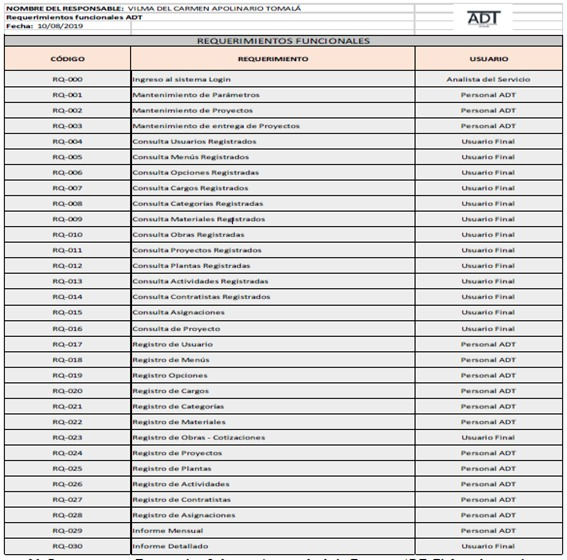
\includegraphics[scale=0.3]{SEGUNDA.jpeg}
\end{figure}


\section*{REQUIRIMIENTOS FUNCIONALES}
\paragraph{Se implementaron los respectivos casos de usos utilizando la herramienta de diagramas de casos de uso para poder establecer la interacción entre el usuario y la plataforma web que se desarrolló para la aplicación.}

\begin{figure}[hbtp]
\caption{}
\centering
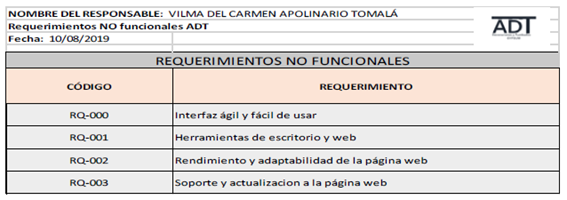
\includegraphics[scale=0.5]{TERCERA.png}
\end{figure}


\begin{figure}[hbtp]
\caption{}
\centering
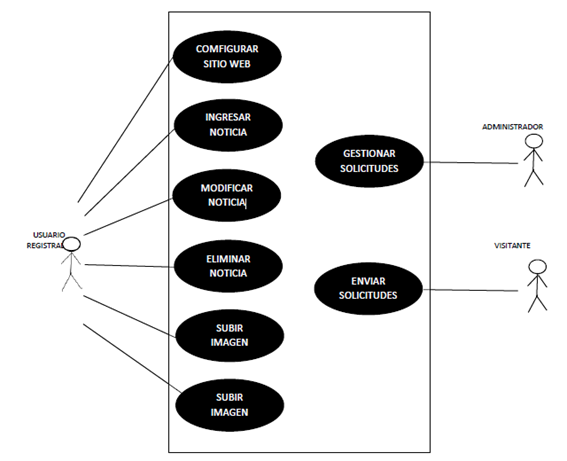
\includegraphics[scale=0.5]{CUARTA.png}
\end{figure}


\section*{Caso de uso para el login y registro del cliente}
\begin{figure}[hbtp]
\caption{}
\centering
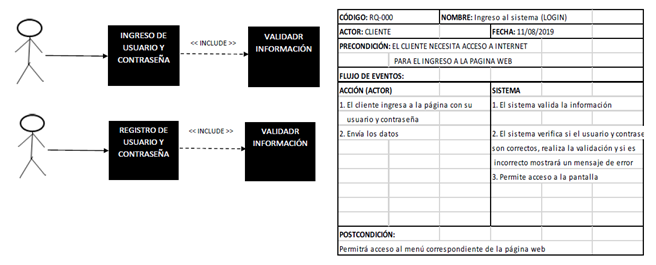
\includegraphics[scale=0.7]{QUINTA.png}
\end{figure}


\section*{Caso de uso Mantenimiento Parámetros}
\begin{figure}[hbtp]
\caption{}
\centering
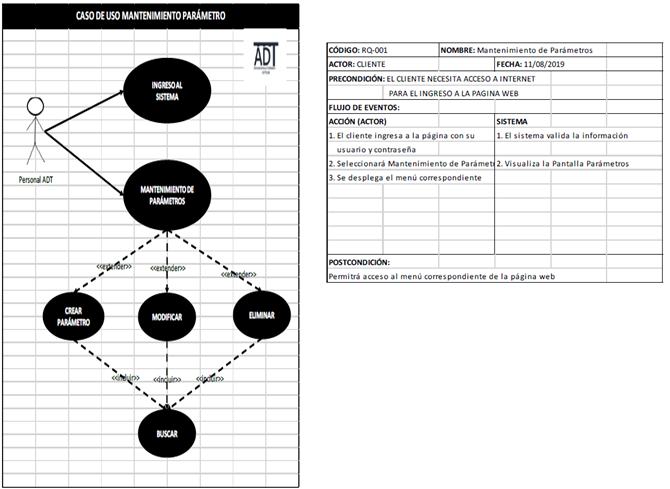
\includegraphics[scale=0.5]{SEXTA.png}
\end{figure}


\section*{Caso de uso registro de usuario}
\begin{figure}[hbtp]
\caption{}
\centering
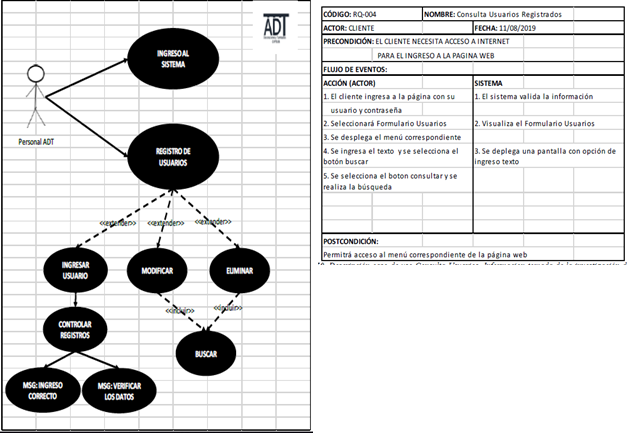
\includegraphics[scale=0.5]{SEPTIMA.png}
\end{figure}


\section*{Caso de uso registro del menú}
\begin{figure}[hbtp]
\caption{}
\centering
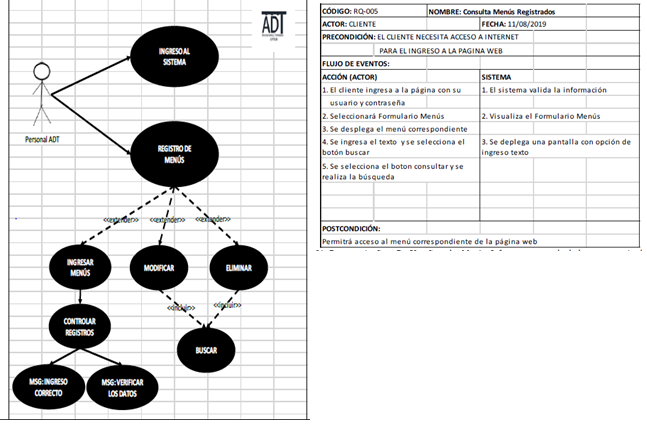
\includegraphics[scale=0.5]{OCTAVA.png}
\end{figure}


\section*{Caso de uso de cargos}
\begin{figure}[hbtp]
\caption{}
\centering
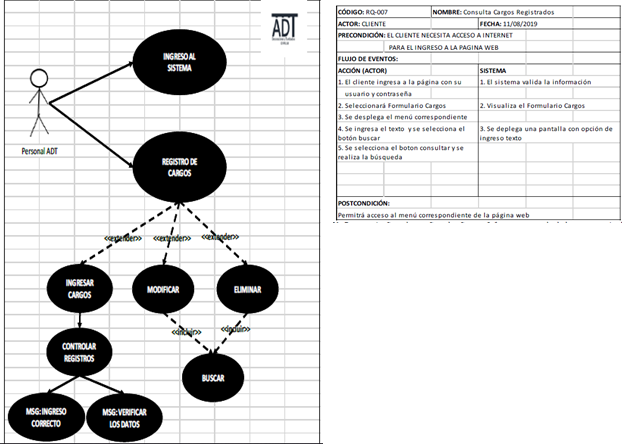
\includegraphics[scale=0.5]{NOVENA.png}
\end{figure}


\section*{Caso de uso registros y cotizaciones}
\begin{figure}[hbtp]
\caption{}
\centering
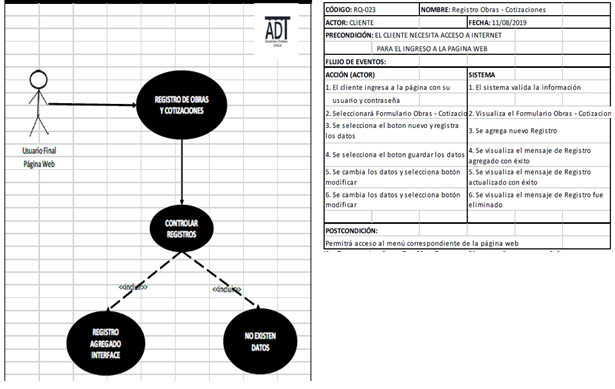
\includegraphics[scale=0.5]{DECIMA.png}
\end{figure}


\section*{Diagrama de clases}
\begin{figure}[hbtp]
\caption{}
\centering
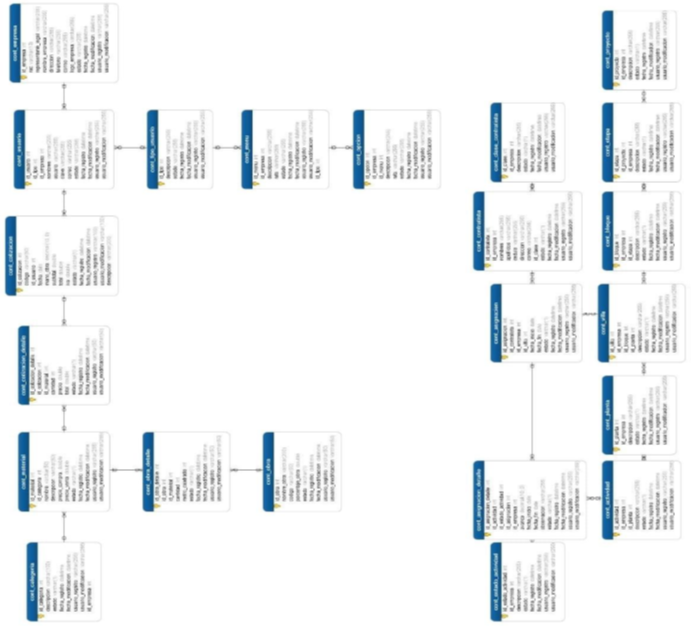
\includegraphics[scale=0.5]{UNDECIMA.png}
\end{figure}


\section*{Diagrama de actividades de parámetros}
\begin{figure}[hbtp]
\caption{}
\centering
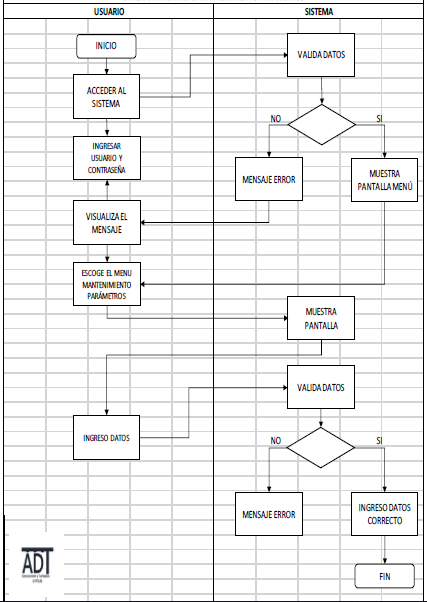
\includegraphics[scale=0.5]{DUODECIMA.png}
\end{figure}


\section*{Mapa del desarrollo de aplicación}
\begin{figure}[hbtp]
\caption{}
\centering
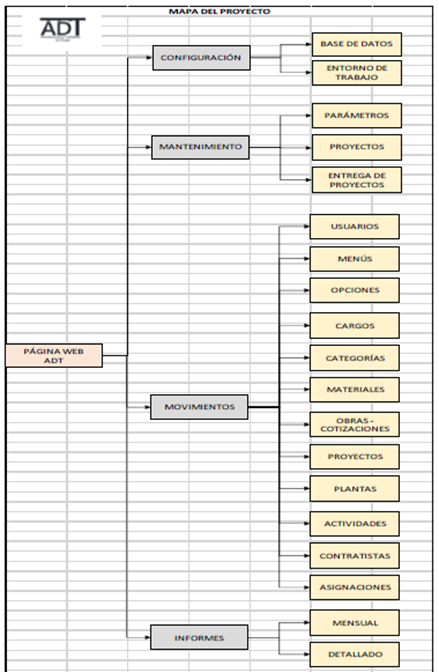
\includegraphics[scale=0.5]{DECIMOTERCERA.png}
\end{figure}


\section*{RESULTADO FINAL}
\begin{figure}[hbtp]
\caption{}
\centering
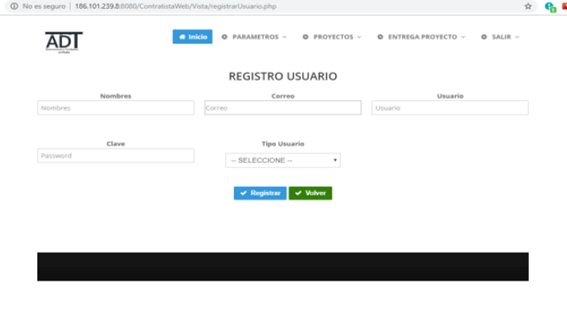
\includegraphics[scale=0.5]{DECIMOCUARTA.png}
\end{figure}


\begin{figure}[hbtp]
\caption{}
\centering
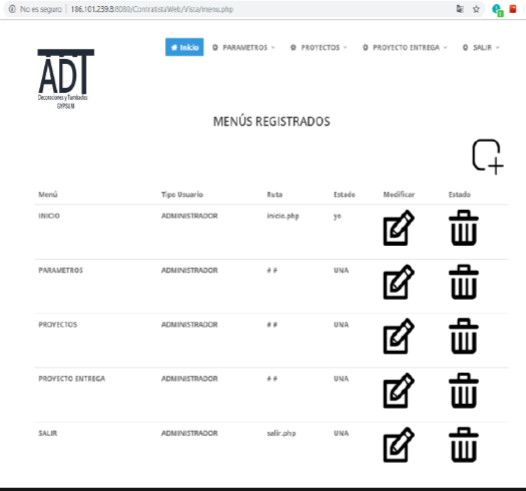
\includegraphics[scale=0.5]{DECIMOQUINTA.png}
\end{figure}


\begin{figure}[hbtp]
\caption{}
\centering
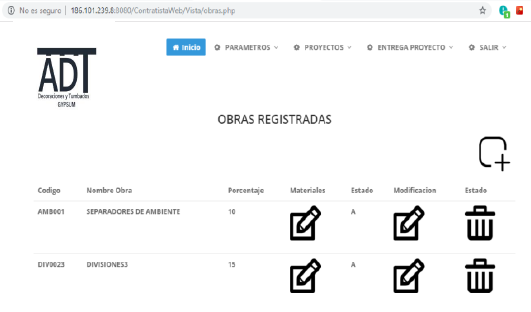
\includegraphics[scale=0.5]{DECIMOSEXTA.png}
\end{figure}


\begin{figure}[hbtp]
\caption{}
\centering
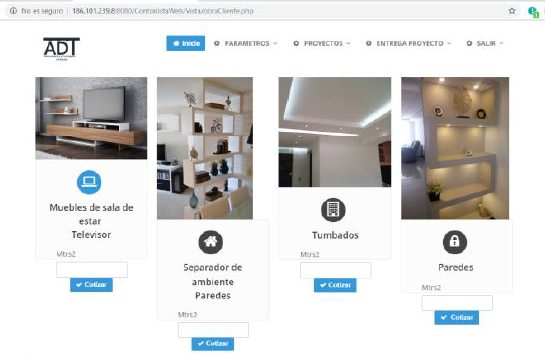
\includegraphics[scale=0.5]{DECIMOSEPTIMA.png}
\end{figure}


\end{document}